%% ----------------------------------------------------------------
\chapter{Chosen Design Approaches}
%% ----------------------------------------------------------------


\section{Camera module}
\label{sec:John_chosen_options}

The camera type chosen was a serial camera as described in \ref{sec:Serial_option}. The particular model chosen was uCam (microCam) or the "Camera Module - Serial JPEG TTL" from the "coolcomponents" website.

The feature set of the uCam is as follows:
	\begin{itemize}
		\item It can output images in both RAW and jpeg formats
		\item It can output RAW images at a range of resolutions:
		\begin{itemize}
			\item 80 x 60
			\item 160 x 120
			\item 320 x 240
			\item 640 x 480
			\item 128 x 128
			\item 128 x 96
		\end{itemize}
		\item It can output jpeg images at a range of resolutions:
		\begin{itemize}
			\item 80 x 64
			\item 160 x 128
			\item 320 x 240
			\item 640 x 480
		\end{itemize}
		\item it can output RAW images with a range of colour settings:
		\begin{itemize}
			\item 2bit Gray Scale
			\item 4bit Gray Scale
			\item 8bit Gray Scale
			\item 8bit Colour
			\item 12bit Colour
			\item 16bit Colour
		\end{itemize}
		\item It will auto-detect baud rates from 14400 to 115200
		\item It has selectable baud rates up to 1228800
		\item Small physical size at 32mm x 32mm
		\item Well documented
	\end{itemize}

The camera was chosen because this feature set meets the specification and also allows for additional functionality, such as setting the resolution, if the full feature set is exploited.

\section{Payload/Ground Station Interaction}

\section{Ground Station Image Viewer}
\subsection{Agreed design}

The final GUI has been planned to have many functions such as auto triggering, image type, resolution type, file path chosen, progress bar, help button, stop and delete.Figure \ref{finalGUI} is the screen shot of the final GUI.

\begin{figure}[!hbtp]
\begin{center}
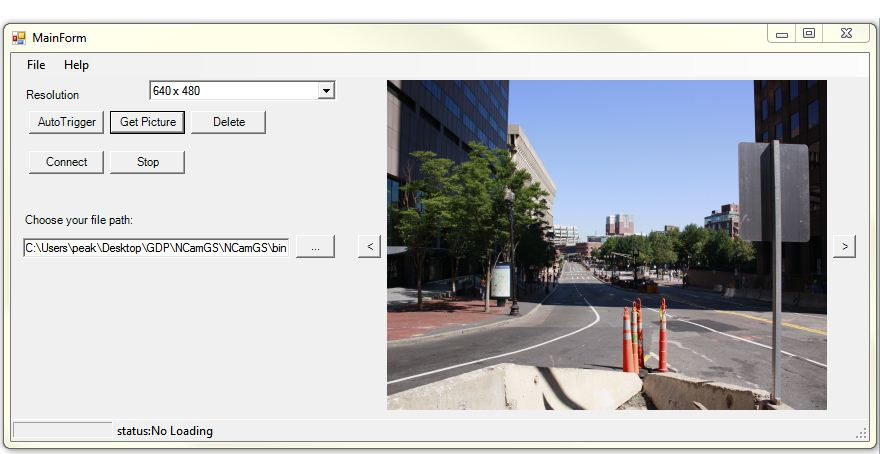
\includegraphics[scale=0.5]{figures/finalGUI.png} 
\end{center}
\caption{final GUI\label{finalGUI}}
\end{figure}
Implementation of the main GUI have omitted some of the buttons in the initial design. The gallery button is not needed because the left and right button is use for scrolling the whole directory of the image. The top tool strip menu has been added because this layout is familiar to any user. The image type have been removed because the raw image data makes the stream data slow and the image viewer program is not supported the file type. The priority is speed of transmitting the data from the UAV. Therefore, raw image is not the option for the user. The progress bar has moved to the button left of the page instead of displaying it below the pictureBox.
This allow the application to have bigger picture box, more compact size and more professional looks.
The stop button allows the user to interrupt the downloading image.
\subsection{Agreed Class Diagram}
The class diagram have been implemented very differently from the planned one. This is because the new plan is to decode it on board and then transmitted to the ground station in JPEG smaller file. Therefore, the class JPEG file reader has changed to C code and to be implemented on board. The DCT class are not needed anymore because all the calculation will be on board. The camera command has taken away as well because the payload will do this  process. The painting class use to draw each pixel onto the pictureBox, but it has not been implemented in the final program because of the stated reason. 
\begin{figure}[!hbtp]
\begin{center}
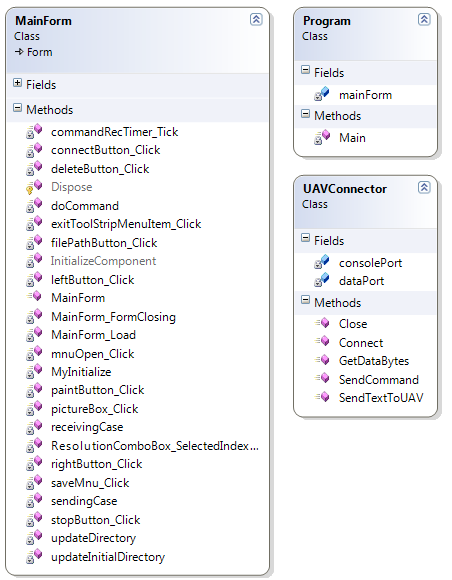
\includegraphics[scale=0.7]{figures/finalClassDiagram.png} 
\end{center}
\caption{Final class diagram of the GUI\label{GUI_finalClassDiagram}}
\end{figure}
\subsection{Agreed Use Case Diagram}
Figure\ref{GUI_finalUseCase} shows an agreed use case diagram. It has changed slightly from the initial use case. The user does not have to control the data stream, this is because the program was planned to do this automatically during the process of getting picture. The type of image can not be chosen because the raw image will be too big and the program can not handle that type of image.

\begin{figure}[!hbtp]
\begin{center}
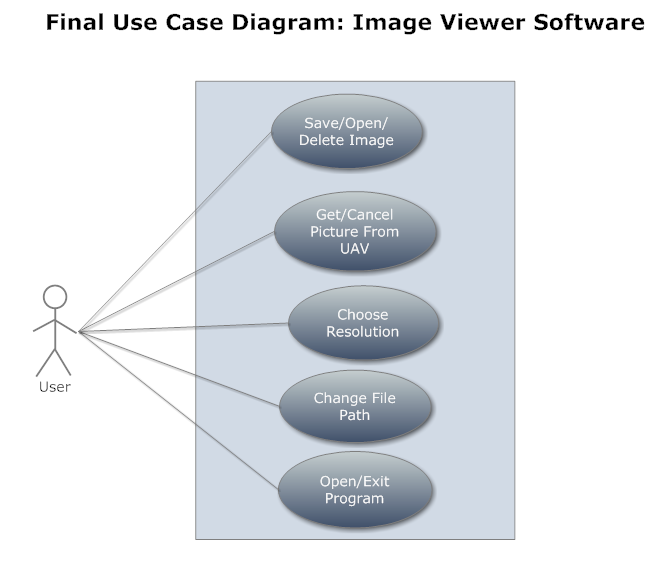
\includegraphics[scale=0.7]{figures/FinaluserCase.png} 
\end{center}
\caption{Final use case diagram of the GUI\label{GUI_finalUseCase}}
\end{figure}

\subsection{.NET C\# class: Socket for the UAV Port Connector}
The socket class was the class chosen for the UAV port connector. It support TCP connection between the client and the server to do low level communication work\cite{xiaX}. The System.IO.Ports namespace has a SerialPort class that can control settings of the port such as baud rate, stop bit, parity bit, and data length. However, this become a disadvantage because the baud rate of the UAV has to be fixed according to the specification. Although it is good to set up a port, but for the software that uses an existing port, the Socket class is more useful and easier to implement by the programmer. The changes of class improve efficiency of connection between port and the program. The baud rate and extra bits are automatically adjusted to be the same as the port, so the setting is identical between the input and output. 

% This is part of the FinalReport document.
% Copyright (C) 2011 Piyabhum Sornpaisarn, Andrew Busse, Michael Hodgson, John Charlesworth, Paramithi Svastisinha
% See the file COPYING in FinalReport/ for copying conditions.

\section{Progressive JPEG Manipulation}

\subsection{JPEG Manipulation}

Prior to knowing the exact speed it would take to send an image from the camera to the ground station, 
it was decided that custom JPEG manipulation would optimize the image further and help reach the target time specified. 
Therefore, tasks concerning the custom manipulation of the JPEG image were planned and worked on at the beginning of the project. 
However, when a working module was constructed, the time needed to send the image was already well within the specified time. 
Because this was the primary advantage of the custom JPEG manipulation process, the task's priority was dropped accordingly.

\subsection{JPEG Data Access}

The dynamic form of data accessing was preferred due to the memory contraints imposed on the device.

\subsection{Entropy-Encoded Data Storage}

The entropy-encoded data will be stored as chrominance pixels for the sake of clarity. 
It is also a method which could be coded more easiliy than seperate component storage. 
This allowed the extractor to work with the progressive JPEG encoder sooner to avoid the task from overrunning.


\section{Physical Implementation}

The physical implementation of the payload has taken many forms, reflecting 
the each of the design-prototype-test cycles that our group experienced.

\begin{itemize}
\item Initially, the system was built in two separate parts: The first was 
the modified version of the ATmega168P-based sample schematic provided by 
our customer, which handled communication to the payload port of the 
autopilot. The second was an Arduino Uno R2 with its Serial (UART) line 
connected to the camera and an SPI connection to an SD card. This system 
simply took an image from the camera and wrote it to the SD card. The SD card 
to Arduino connection was via some protoboard and an SD card reader breakout 
board on loan from Zepler Stores.
\item The next design iteration used an "Il Matto" board and daughter board, 
designed for 2011's D4 lab (a two-week Design and Build exercise for second 
year Electronic Engineers). The board itself is rather simple - an ATmega644P 
with all of its ports connected to expansion headers, an SPI line connection 
to an SD card reader, and power taken from a mini-USB connection, stepped 
down to 3V3 by a linear regulator. A daughter board (which slots into the 
expansion headers) has the transceiver to communicate with the autopilot

This implementation of the payload contains all the elements of the final 
schematic, so technically could be test-flown.
\item Whereas the above approach would technically fulfil the specification, 
implementing it would be expensive: the Il Matto boards were one-off boards 
designed specifically for a lab, so a customer would certainly need to 
manufacture and build their own, including the daughter board. Having this as 
a single PCB solution would be a lot neater, smaller, lighter and cheaper.

Therefore, a final PCB was designed (this is elaborated upon in 
\ref{sec:PCB-implementation}), specific to our application, with all the 
features we need. Only through-hole components are used where possible, 
making the task of soldering components to the PCB as easy as possible.
\end{itemize}

\section{System Design Overview}

